\documentclass[10pt]{article}
\usepackage[utf8]{inputenc}
\usepackage[T1]{fontenc}
\usepackage{hyperref}
\usepackage{bookmark}
\usepackage{lipsum} % for placeholder text, remove if not needed
\usepackage[a4paper, portrait, margin=1.5cm]{geometry}
\usepackage{graphicx}
\usepackage{fancyhdr}
\usepackage{float}
\usepackage{color}
\usepackage{subcaption}
\usepackage{parskip}
\usepackage{setspace}
\usepackage{amsmath}
\definecolor{orange}{rgb}{1,0.5,0}

\title{\textbf{A mobile application for augmenting technical documentation using AR and AI}}
\author{\large Ani Bitri\\ Dr. Paris Giampouras, John McNamara\\ University of Warwick and IBM}



\begin{document}

\thispagestyle{empty}

\begin{spacing}{2}
	\begin{center}
        \begin{figure}
            \begin{subfigure}[b]{0.45\textwidth}
                \centering
                
\includegraphics[height=4cm]{img/WarwickCrest.png}
                \label{fig:WarwickCrest}
            \end{subfigure}
            \hfill
            \begin{subfigure}[b]{0.45\textwidth}
                \centering
                
\includegraphics[height=4cm]{img/IBM_Logo.png}
                \label{fig:IBM_Logo}
            \end{subfigure}
        \end{figure}
	\end{center}
	\vspace{5mm}
	\begin{center}
		\textbf{\begin{LARGE}
		A mobile application for augmenting technical documentation using AR and AI
		\end{LARGE}}
		\vspace{5mm}
	\end{center}
	\begin{center}
		{\large CS310: Third Year Project}\\
		\vspace{10mm}
	\end{center}
	\begin{center}
		\textbf{\large Ani Bitri}
		\vspace{10mm}
	\end{center}
	\begin{center}
	     {\large Supervisors: Dr. Paris Giampouras, John McNamara}\\
		\textbf{\large Department of Computer Science}\\
		{\large University of Warwick and IBM}\\
		{\large October 2025\\}
	\end{center}
\end{spacing}

\newpage

\section{Requirements}
    \subsection{Functional Requirements}
=
    \begin{enumerate}
        \item \textbf{Augmented Reality System:}
            \begin{itemize}
                \item FR-1: The system shall allow users to open the camera interface within the mobile application to scan technical documents.
                \item FR-2: The system shall allow the user to upload technical documents from their device storage.
                \item FR-3: The system shall recognize diagrams, images, flowcharts, and schematics within the scanned or uploaded documents using image recognition techniques.    
                \item FR-4: The backend shall extract diagram elements and textual information from the recognized diagrams using IBM Granite Vision.
                \item FR-5: The system shall generate interactive AR overlays that provide explanations of components, relationships, and interactions within the diagrams.
                \item FR-6: The system shall allow users to interact with the AR overlays to explore additional information about the diagram components and their relationships.
                \item FR-7: The system shall provide visual cues to confirm successful recognition and overlay placement.
            \end{itemize}
        \item \textbf{AI Assistant:}
            \begin{itemize}
                \item FR-8: The system shall allow users to input natural language queries related to the scanned or uploaded technical documents.
                \item FR-9: The backend shall use the Granite AI model to process user queries and generate relevant responses based on the document content.
                \item FR-10: The AI shall combine diagram data from Granite Vision with textual information from the documents to provide comprehensive answers.
                \item FR-11: The system shall display the AI-generated responses within the mobile application
                \item FR-12: The AI assistant shall retain context from previous interactions to provide coherent and relevant responses.
            \end{itemize}
        \item \textbf{Data Management and Communication:}
            \begin{itemize}
                \item FR-13: The app shall communicate with the backend over HTTPS with token-based authentication to ensure secure data transmission.
                \item FR-14: The backend shall handle user requests, forward images to IBM Granite Vision, combine results with IBM Granite AI, and return structured JSON responses to the mobile app.
                \item FR-15: The system shall implement caching mechanisms to store previously processed diagrams and AI responses for improved performance.
                \item FR-16: The system shall log user interactions and queries for analytics and improvement purposes.
                \item FR-17: The system shall provide error handling mechanisms to manage failures in image recognition, AI processing, or network connectivity, and inform users appropriately.
            \end{itemize}
        \item \textbf{User Interface and Experience:}
            \begin{itemize}
                \item FR-18: The mobile application shall present a home screen with navigation options to access camera view, document upload, AI assistant, and settings.
                \item FR-19: The system shall provide an interactive chat interface for AI interactions, showing both user queries and AI responses in a conversational format.
                \item FR-20: Users shall be able to switch between text input, speech input and AR interaction modes seamlessly.
            \end{itemize}
    \end{enumerate}

\section{System Architecture}
Provide a high-level overview of the system architecture. Include diagrams where appropriate to illustrate the system components and their interactions.

    \subsection{Design Pattern}

    The design pattern which will be adopted for this project is the Model-View-ViewModel (MVVM) pattern. This pattern is well-suited for applications that require a clear separation
    of concerns between the user interface and logic, making it easier to manage and test the application. Furthermore, the MVVM pattern facilitates a more modular and maintainable
    codebase, which is essential for the iterative development process planned for this project. The image below illustrates the MVVM architecture which will be used in the project.

    \begin{figure}[H]
        \centering
        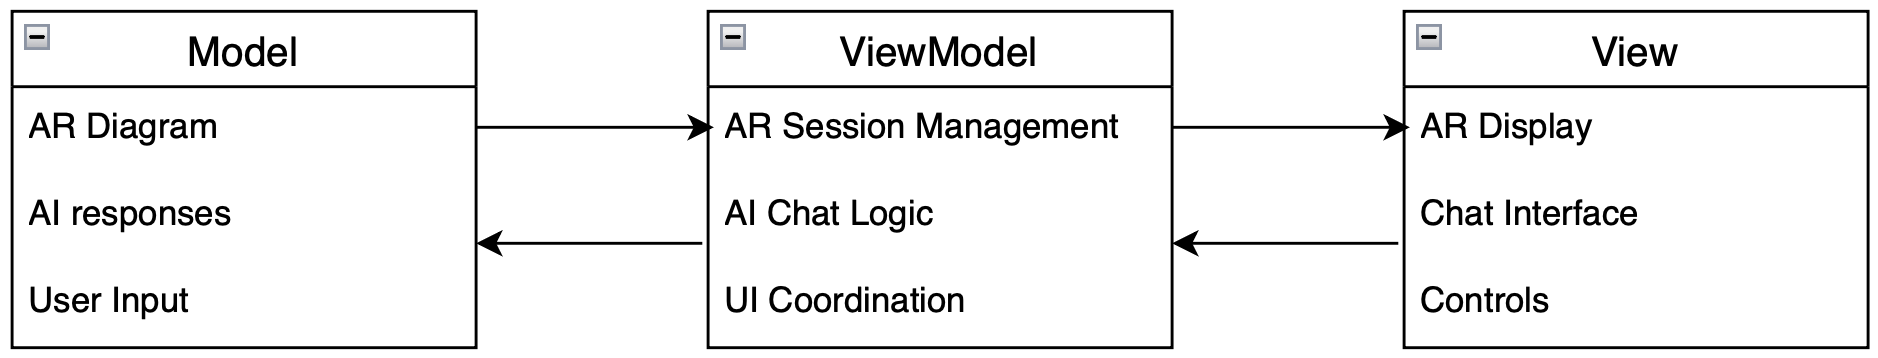
\includegraphics[width=\textwidth]{img/Pattern.png}
        \caption{MVVM Architecture Pattern}
        \label{fig:Pattern}
    \end{figure}

    \subsection{Frontend Design}

    \subsubsection{User Interface and User Experience}

        The application will feature a user-friendly interface that allows users to easily navigate through the app and access its features. The UI will be designed to be intuitive and responsive, ensuring a seamless user experience. When the user open the app, they will be presented with
        a simple home screen with options to scan a document, upload a document or access the history of previously scanned documents. Besides the home screen, the app will also include a tab for the chatbot, where users can interact with the AI assistant, and a settings tab for configuring
        app preferences. The image below illustrates the proposed UI design for the application:

        \begin{figure}
            \centering
            \begin{subfigure}{0.3\textwidth}
                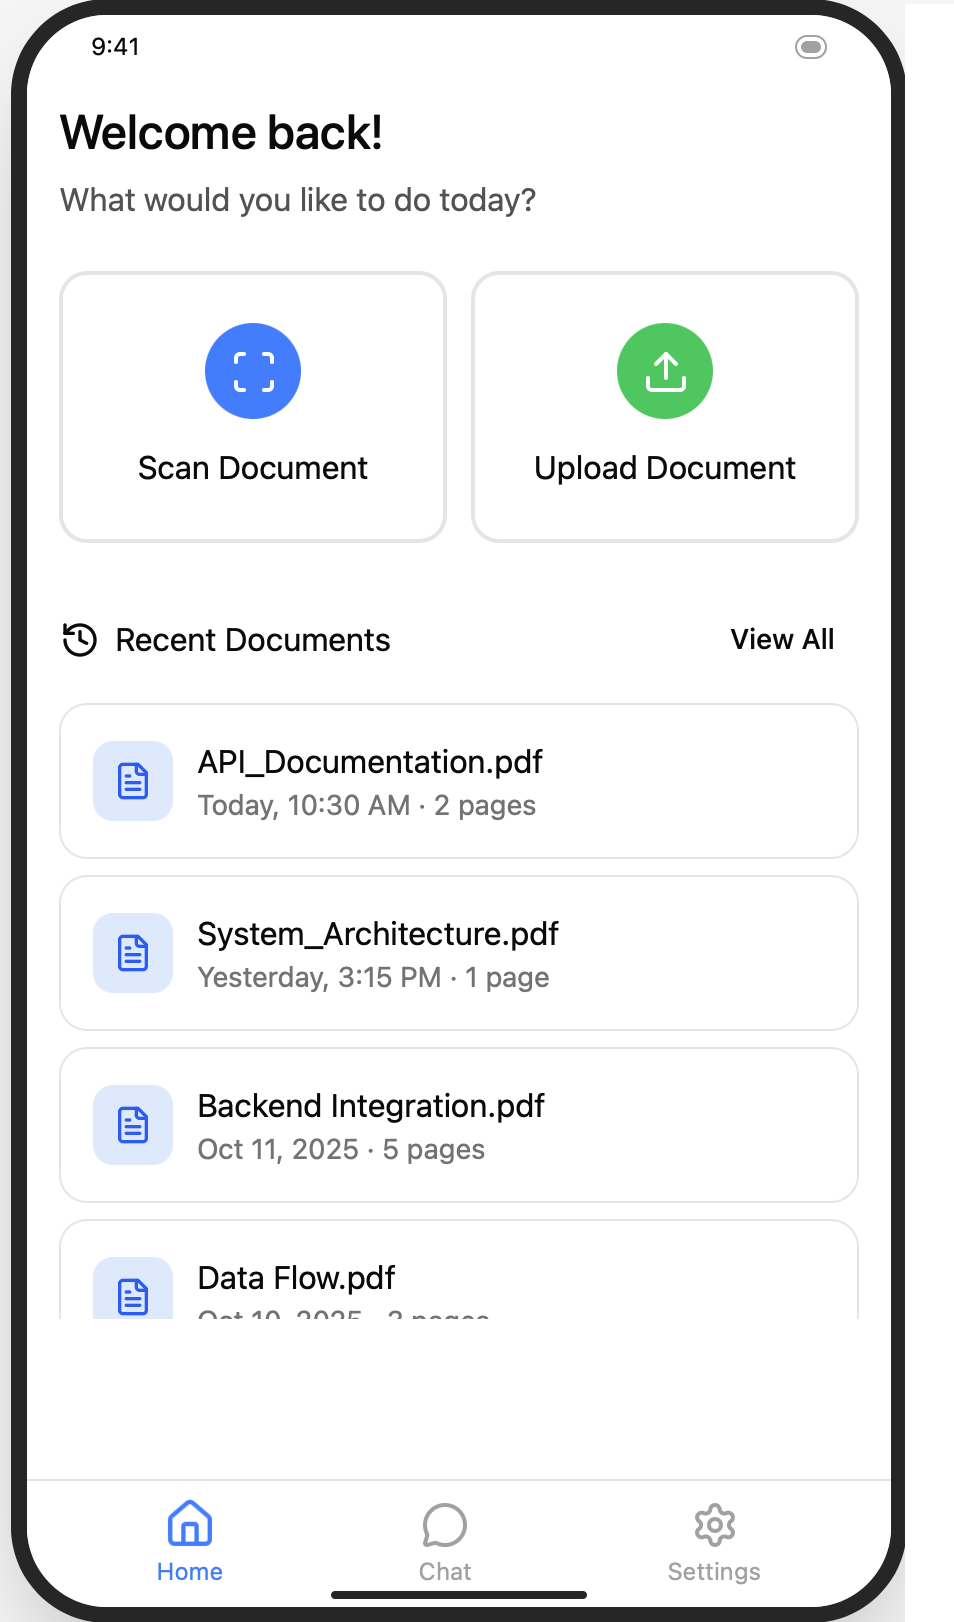
\includegraphics[width=\textwidth]{img/FrontendHomeTab.png}
                \caption{Home Screen}
                \label{fig:HomeScreen}
            \end{subfigure}
            \hfill
            \begin{subfigure}{0.3\textwidth}
                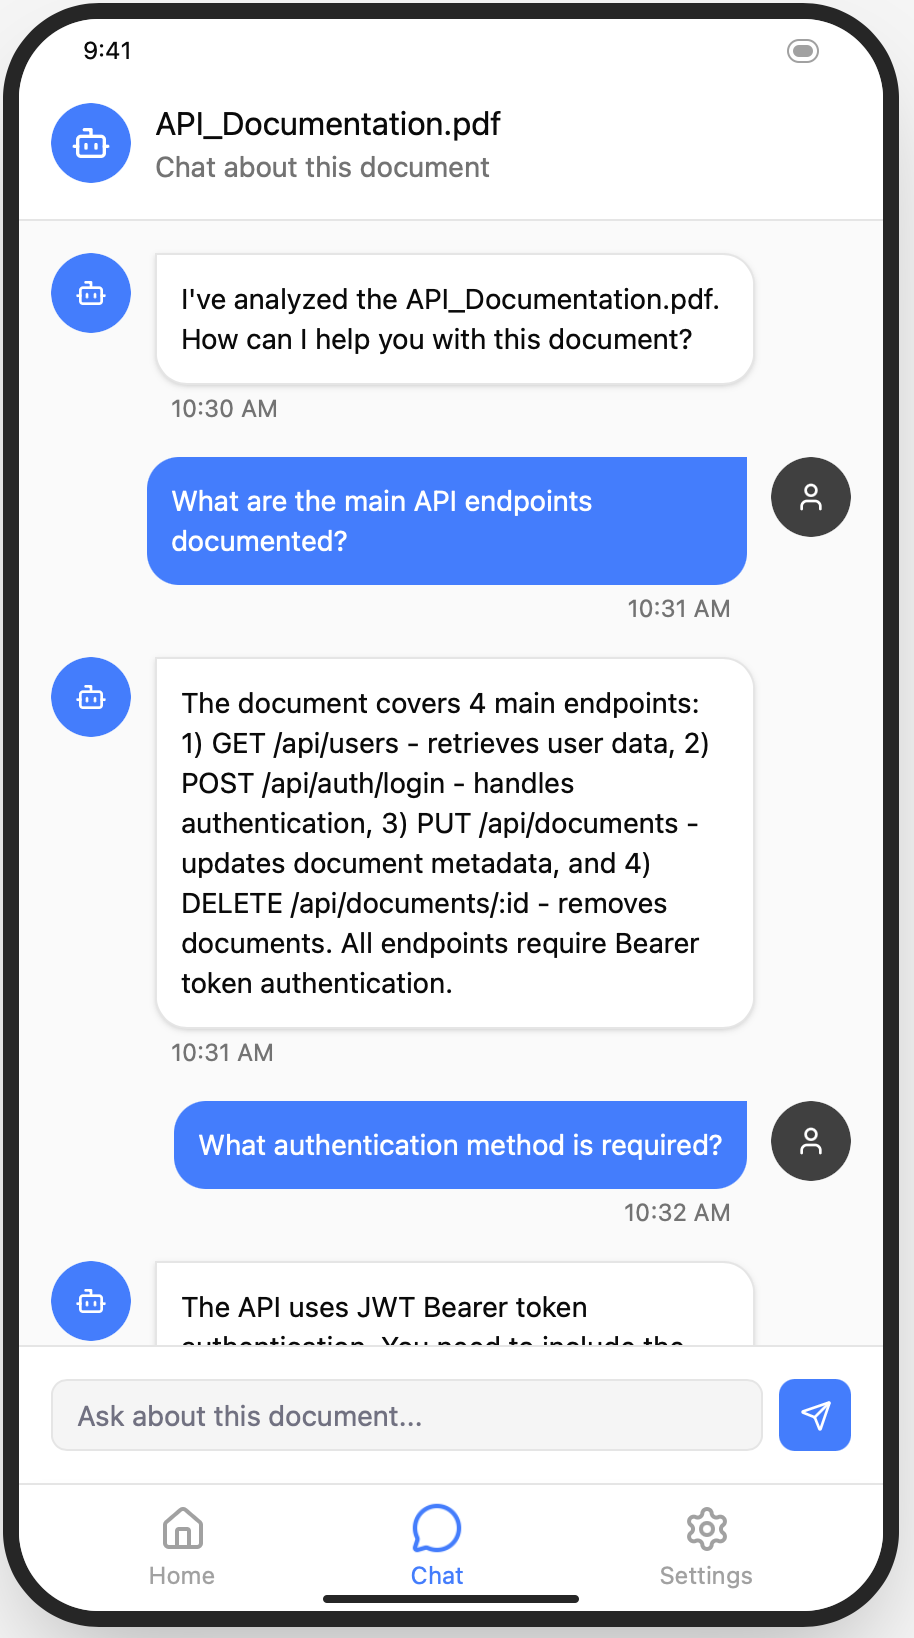
\includegraphics[width=\textwidth]{img/FrontendChatTab.png}
                \caption{Chatbot Tab}
                \label{fig:ChatbotTab}
            \end{subfigure}
            \hfill
            \begin{subfigure}{0.3\textwidth}
                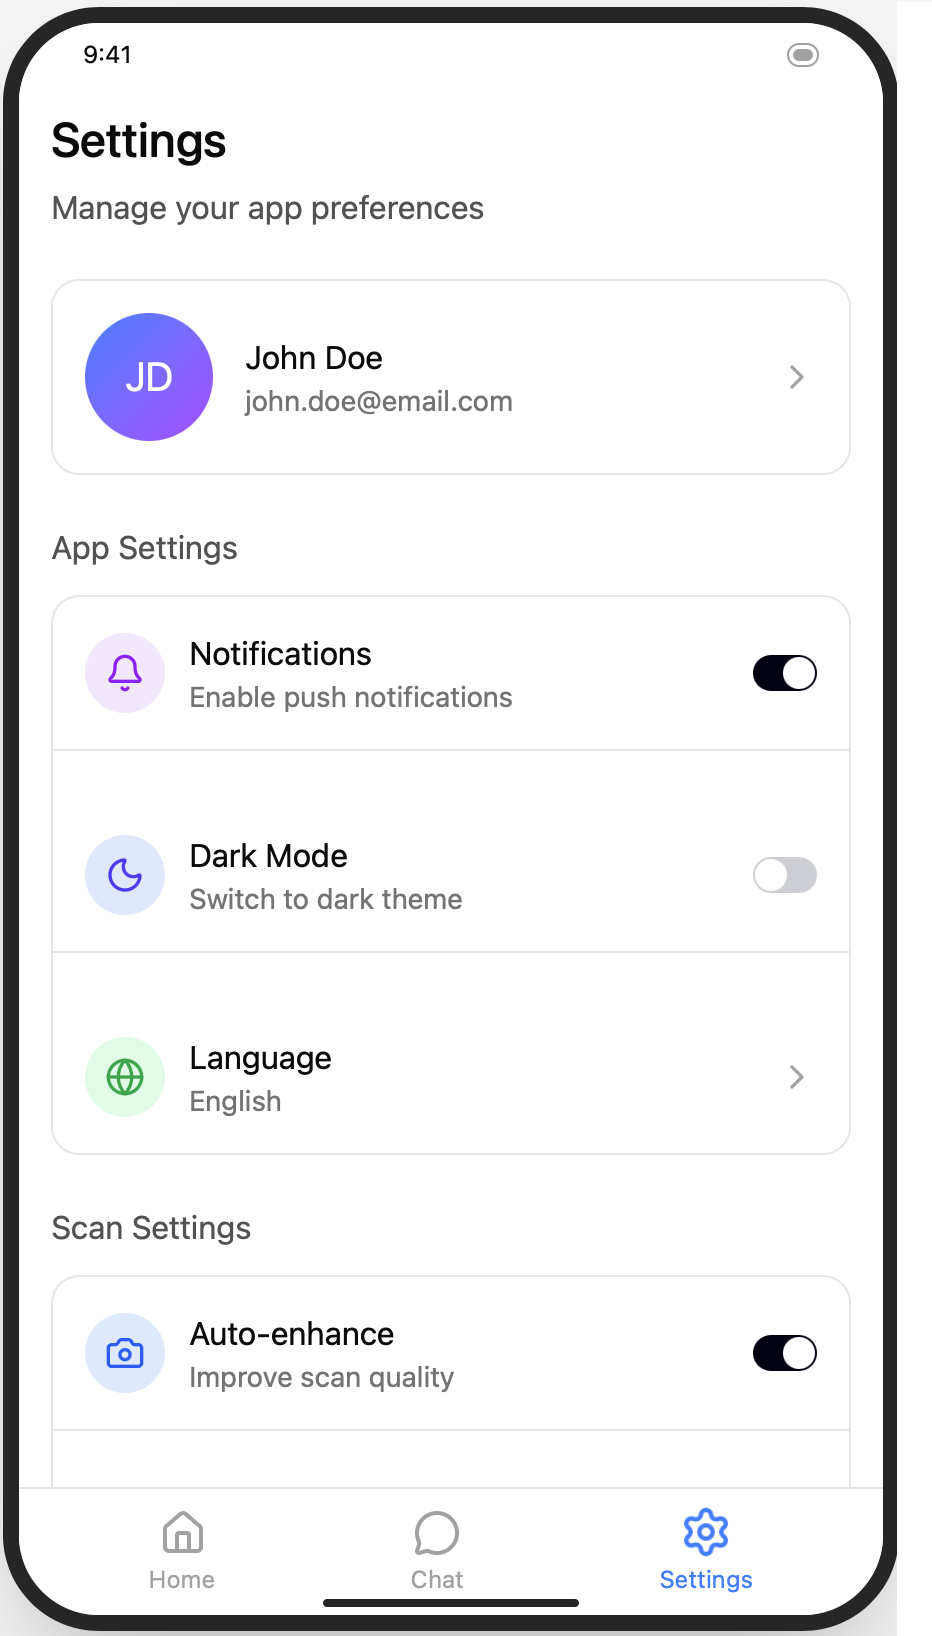
\includegraphics[width=\textwidth]{img/FrontendSettingsTab.png}
                \caption{Settings Tab}
                \label{fig:SettingsTab}
            \end{subfigure}
            \caption{Proposed UI Design for the Application}
            \label{fig:UIDesign}
        \end{figure}

    Upon selecting the scan option, the user will be directed to the camera interface, where they can capture pictures of the technical documentation. Alternatively, the user can choose to upload the document from their device's storage and access the same features. After scanning or uploading
        a document, the app will process the text, images and diagrams, and give the user the option to view the AR overlays or interact with the AI assistant. The AR overlays will provide interactive elements that explain components, relationships and interactions within the diagrams based on the user's
        input and the information extracted from the document. The image below illustrates a flow chart of the app's user interface and navigation:

        % Flowchart image here
    \subsubsection{Error Handling and Feedback}

        To ensure a smooth user experience, the application will include robust error handling mechanisms. Internal errors will be handled gracefully and automatically, with appropriate messages displayed to the user upon interruptions. For example, if the app fails to recognize a diagram or if the AI assistant
        cannot process a query, the user will be informed of the issue and provided with suggestions for resolution. External errors will be handled by providing informative error messages to guide users in case of issues such as failed scans or uploads, network connectivity problems or AR tracking errors. Furthermore,
        error prevention strategies will be implemented to minimize their occurrence and impact on the user experience. Such strategies include input validation, network status checks and AR tracking optimizations. This approach will ensure that users can effectively utilize the app's features without being hindered by technical issues.



    \subsubsection{Integration with Backend and Data Flow}

        The frontend of the application will communicate with the backend services to process the scanned or uploaded documents and retrieve relevant information. The data flows as follows:
        \begin{enumerate}
            \item The user scans or uploads a document using the app's interface.
            \item The frontend validates the input and sends the document data to the backend for processing.
            \item The validated data is sent to the backend services for text recognition, diagram analysis and AI processing.
            \item The backend processes the data and generates AR overlays and AI responses based on the document content.
            \item The generated AR overlays and AI responses are sent back to the frontend for display to the user.
            \item The user interacts with the AR overlays and AI assistant, and any further queries or actions are sent back to the backend for processing.
        \end{enumerate}
        
    \subsection{Backend Design}

        \subsubsection{Overview}

            The backend of the application will act as the intelligence and coordination layer that connects the React Native frontend to IBM's AI services. Its primary function is to process
            the scanned or uploaded documents and other user inputs, understand their content, and generate appropriate AR overlays and AI responses. The backend ensures that heavy computational
            tasks are offloaded from the mobile device, providing a seamless user experience.

        \subsubsection{Workflow}

        The backend workflow consists of several key steps:
        \begin{enumerate}
            \item \textbf{Request Reception:} The backend receives the scanned images or uploaded from the frontend via RESTful API calls.
            \item \textbf{Image and Data Processing:}
                \begin{itemize}
                    \item If an image is recieved, it is processed using IBM Granite Vision to extract text and identify diagrams, returning structured data.
                    \item If text data is recieved, it is analyzed to identify key components, relationships and interactions.
                \end{itemize}
            \item \textbf{AI Reasoning and Response Generation:} The backend composes of a prompt that combines:
                \begin{itemize}
                    \item Extracted diagram information from IBM Granite Vision.
                    \item Relevant documentation snippets.
                    \item The user's query or interaction context.
                \end{itemize}

                The composite prompt is sent to IBM Granite, which then generates a natural language response.
            \item \textbf{Response Delivery:} The backend merges the AI-generated response with structured metadata and send a single JSON payload back to the mobile app. The fronted then
            displays the AR overlays and AI responses to the user.
        \end{enumerate}

        \subsubsection{Data Management and Caching}
            To improve efficiency, the backend implements:
            \begin{itemize}
                \item \textbf{Caching:} Previously processed diagrams are stored to reduce redundant processing using Redis or local storage.
                \item \textbf{Error Handling:} AI or network failures return structured JSON error messages to the frontend for user notification.
                \item \textbf{User session logs:} Stored in a database for analytics and improvement (PostgreSQL or Firebase).
            \end{itemize}
            
    \subsection{Technology Stack}
        The project will utilize the following technologies:
        \begin{itemize}
            \item \textbf{Frontend:} React Native for cross-platform mobile development, ARCore/ARKit/ViroReact for augmented reality functionalities.
            \item \textbf{Backend:} Node.js with Express for server-side logic, IBM Granite 4.0 for AI capabilities, IBM Granite Vision for image recognition, and MongoDB for data storage.
            \item \textbf{Development Tools:} Visual Studio Code for code editing, Git for version control, REST APIs for communication between frontend and backend.
        \end{itemize}




\end{document}